 \documentclass[pdftex,12pt, oneside]{article}

%\usepackage[paperwidth=8.5in, paperheight=13in]{geometry} % Folio
\usepackage[paperwidth=8.27in, paperheight=11.69in]{geometry} % A4

\usepackage{makeidx}         % allows index generation
\usepackage{graphicx}        % standard LaTeX graphics tool
                             % when including figure files
\usepackage[bottom]{footmisc}% places footnotes at page bottom
\usepackage[english]{babel}
\usepackage{enumerate}
\usepackage{paralist}
\usepackage{float}
\usepackage{gensymb}  
\usepackage{listings}
\usepackage{color}
\usepackage{mathtools} % atau \usepackage{amsmath}
\renewcommand{\baselinestretch}{1.5}

\newcommand{\HRule}{\rule{\linewidth}{0.5mm}}

\definecolor{codegreen}{rgb}{0,0.6,0}
\definecolor{codegray}{rgb}{0.5,0.5,0.5}
\definecolor{codepurple}{rgb}{0.58,0,0.82}
\definecolor{backcolor}{rgb}{0.95,0.95,0.92}

\lstdefinestyle{mystyle}{
  backgroundcolor=\color{backcolor},
  commentstyle=\color{codegreen},
  keywordstyle=\color{magenta},
  stringstyle=\color{codepurple},
  basicstyle=\footnotesize,
  breakatwhitespace=false,
  breaklines=true,
  captionpos=b,
  keepspaces=true,
  numbers=left,
  numbersep=5pt,
  showspaces=false,
  showstringspaces=false,
  showtabs=false,
  tabsize=2
}

\lstset{style=mystyle}


\begin{document}
\sloppy % biar section ga melebar melewati kertas

\begin{center}
{\large DOKUMENTASI RANCANGAN SISTEM JARINGAN KOMPUTER - SIMPATDA}
\\[1cm]
11 Januari 2017\\
Priyanto Tamami, S.Kom.
\end{center}

%\frontmatter%%%%%%%%%%%%%%%%%%%%%%%%%%%%%%%%%%%%%%%%%%%%%%%%%%%%%%


%%%%%%%%%%%%%%%%%%%%%%%%%%%%%%%%%%%%%%%%%%%%%%%%%%%%%%%%%%%%%%%%%%%%%%

\section{ANALISIS KEBUTUHAN}

\subsection{PENDAHULUAN}

Dengan dilakukannya perubahan struktur kedinasan, maka dibutuhkan penyesuaian terhadap struktur jaringan komputer, terutama dalam pelaksanaan kegiatan operasional administrasi pajak daerah. 

Beberapa aplikasi yang nantinya akan dapat diakses oleh dua bidang pengelola pendapatan daerah yaitu, SISMIOP, Simpatda, dan Simda Pendapatan.

\subsection{METODE ANALISIS KEBUTUHAN}

Pemilihan metode analisis kebutuhan yang diterapkan kali ini yaitu : observasi dan analisa prosedur.

Rincian metodenya adalah sebagai berikut :

\textbf{Obervasi}

Ini dilakukan dalam rangka pengamatan kondisi fisik ruangan, berapa panjang kabel jaringan yang diperlukan, lokasi \textit{switch} atau \textit{router} yang diperlukan, lokasi \textit{server}, dan ketersediaan perlengkapan untuk membangun jaringan.

\textbf{Prosedur Analisis}

Ini dilakukan untuk menentukan topologi jaringan yang cocok untuk melakukan komunikasi data, termasuk pembagian jaringan sebagai strategi untuk melakukan deteksi kegagalan sistem.

\subsection{ANALISA DAN SIMPULAN}

Hasil dari kegiatan analisa adalah bahwa dalam pengelolaan pajak daerah akan menggunakan beberapa sistem informasi, yaitu sebagai berikut :

\begin{enumerate}[1.]
  \item SISMIOP, yaitu sistem informasi manajemen objek pajak khusus untuk pengelolaan Pajak Bumi dan Bangunan Perdesaan dan Perkotaan. Sistem ini berbentuk \textit{client server} sehingga aplikasi harus dipasangkan (\textit{install}) pada komputer \textit{client} agar sistem dapat digunakan.
  
  \item Simpatda, yaitu sistem informasi yang digunakan untuk mengelola jenis pajak daerah lain selain PBB-P2 dan BPHTB, Simpatda ini rencananya sudah tidak digunakan lagi di tahun 2017.
  
  \item Simda Pendapatan, yaitu sistem informasi yang digunakan untuk menggantikan Simpatda yang nantinya sudah tidak digunakan lagi.
\end{enumerate}

Sistem-sistem informasi tersebut harus dapat digunakan oleh kedua bidang yang menangani pajak daerah, sehingga perlu dilakukan penyesuaian terhadap jaringan komputer yang sudah ada.

Karena alamat jaringan yang berbeda antara bidang Pendataan dan Penetapan dengan bidang Penagihan dan Pelaporan, maka dibutuhkan \textit{router} untuk menghubungkannya agar dapat saling berkomunikasi.

\section{STUDI KELAYAKAN}

\subsection{MASALAH}

Dari hasil analisia, bahwa jaringan antara dua bidang memiliki alamat jaringan yang berbeda, sehingga diperlukan sebuah \textit{router} untuk menjembatani komunikasi antara kedua jaringan yang berbeda ini.

\subsection{LINGKUNGAN IMPLEMENTASI}

Lingkungan implementasi untuk sistem jaringan komputer yang dibutuhkan hanya bersifat lokal antar bidang, dimana \textit{server} SISMIOP berada pada bidang Pendataan dan Penetapan, sedangkan \textit{server} Simpatda dan Simda Pendapatan berada pada bidang Penagihan dan Pelaporan.

\subsection{REKOMENDASI}

Rekomendasi yang dapat diberikan adalah menggunakan koneksi jaringan komputer dengan kabel UTP, karena koneksi menggunakan kabel UTP cukup stabil dan cepat, dimana jarak antara bidang Pendataan dan Penetapan dengan bidang Penagihan dan Pelaporan jaraknya tidak terlalu jauh. Rekomendasi ini juga tidak terlepas dari kondisi jaringan LAN yang sudah stabil di kedua bidang.

\subsection{KONFIGURASI SISTEM ALTERNATIF}

Sistem alternatif yang dapat digunakan adalah koneksi jaringan internet. Namun konfigurasi dengan cara ini sangat bergantung dengan kualitas jaringan internet, bila ada permasalahan dengan jaringan internet, maka aplikasi tidak akan dapat digunakan sampai perbaikan selesai oleh pihak penyedia jaringan internet.

\subsection{RUANG LINGKUP SISTEM}

Ruang lingkup dari sistem ini tidak terlepas dari lingkungan implementasi jaringan komputer diterapkan, yaitu hanya menghubungkan koneksi jaringan pada dua bidang dengan dua alamat jaringan yang berbeda. Nantinya jaringan akan terhubung dengan \textit{switch} di bidang Penagihan dan Pelaporan, dan terhubung dengan \textit{router} di bidang Pendataan dan Penetapan.

\subsection{KELAYAKAN SISTEM}

Dari aspek teknologi, maka sistem yang akan dikembangkan mampu mengakomodir komunikasi jaringan komputer pada dua bidang, dimana tiap bidang dapat melakukan akses ke aplikasi masing-masing.

Dari aspek operasional, SDM / operator yang mengoperasikan aplikasi perlu adaptasi, bagi pegawai dari bidang PBB dan BPHTB dulunya mungkin sudah terbiasa dengan SISMIOP untuk manajemen data subjek dan objek pajak PBB-P2, sehingga perlu adaptasi dengan aplikasi Simpatda dan Simda Pendapatan, begitu pula sebaliknya, pegawai dari bidang Pajak Daerah dan Pendapatan Lain-lain perlu beradaptasi dengan SISMIOP.

\subsection{SIMPULAN}

Sebagaimana rekomendasi dari studi kelayakan pembangunan jaringan komputer diatas, maka komunikasi yang nantinya terbentuk antar jaringan melalui media kabel UTP, dengan alternatif berupa jaringan internet.

\section{METODE KOMUNIKASI}

Metode yang digunakan untuk komunikasi data antar komputer adalah dengan protokol TCP/IP. Komunikasi antara \textit{client} dan \textit{server} pada aplikasi SISMIOP tetap menggunakan \textit{port} 1521, aplikasi Simda Pendapatan nantinya akan menggunakan \textit{port default} milik basis data Microsoft SQL Server yaitu 1433. Sedangkan aplikasi Simpatda berupa aplikasi \textit{web-based} sehingga cukup diakses menggunakan \textit{browser} di alamat 192.168.17.100.

\section{TOPOLOGI JARINGAN}

Topologi jaringan yang cocok digunakan adalah model \textit{Tree} (Pohon), dengan penerapan pada dua alamat jaringan yang berbeda, artinya, bila ada kesalahan saat melakukan komunikasi dengan posisi \textit{server} berada pada lintas bidang, maka dapat dipastikan ada gangguan pada kabel penghubung antar bidang.

\section{DIAGRAM JARINGAN}

Diagram jaringan untuk menggambarkan jaringan yang terbentuk adalah seperti terlihat pada gambar \ref{fig:dia-jaringan} :

\begin{figure}[H]
  \centering
  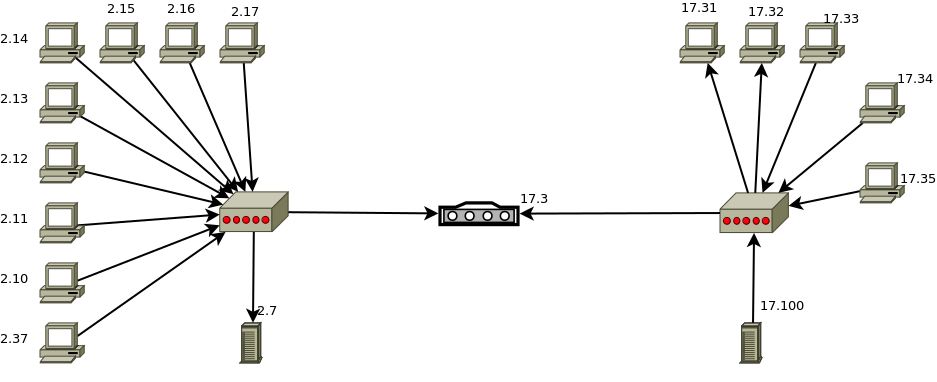
\includegraphics[width=1\textwidth]{./resources/dia-jaringan}
  \caption{Diagram Jaringan Pajak Daerah}
  \label{fig:dia-jaringan}
\end{figure}

Kondisi \textit{server} SISMIOP berada pada alamat 2.7, sedangkan \textit{server} Simpatda berada pada alamat 17.100.

\textit{Client} dari alamat jaringan 2.0 dapat mengakses \textit{server} Simpatda dengan langsung melakukan akses ke alamat 17.100 dengan \textit{browser}, sedangkan \textit{client} dari alamat 17.0 dapat mengakses SISMIOP di alamat 17.3.

\section{PERANGKAT KERAS DAN PERANGKAT LUNAK JARINGAN}

Perangkat keras yang digunakan untuk membangun jaringan komputer pajak daerah di kedua bidang ini adalah kabel UTP Cat 5e berikut konektor RJ45, 2 (dua) unit \textit{switch} yang telah terpasang, dan 1 (satu) unit \textit{router} yang sebetulnya difungsikan sebagai \textit{gateway} untuk menghubungkan dua jaringan di dua bidang. 

Jumlah komputer \textit{client} yang terhubung pada jaringan ini ada 14 (empat belas unit), dengan 2 (dua) unit \textit{server}.

Perangkat lunak yang digunakan dalam jaringan komputer ini yang perlu konfigurasi hanya dari \textit{router} atau \textit{gateway} Cisco RV042G dengan konfigurasi untuk \textit{interface} WAN2 menggunakan \textit{static IP}. Konfigurasi pada perangkat Cisco RV042G dapat dilihat pada gambar \ref{fig:konfig-cisco} :

\begin{figure}[H]
  \centering
  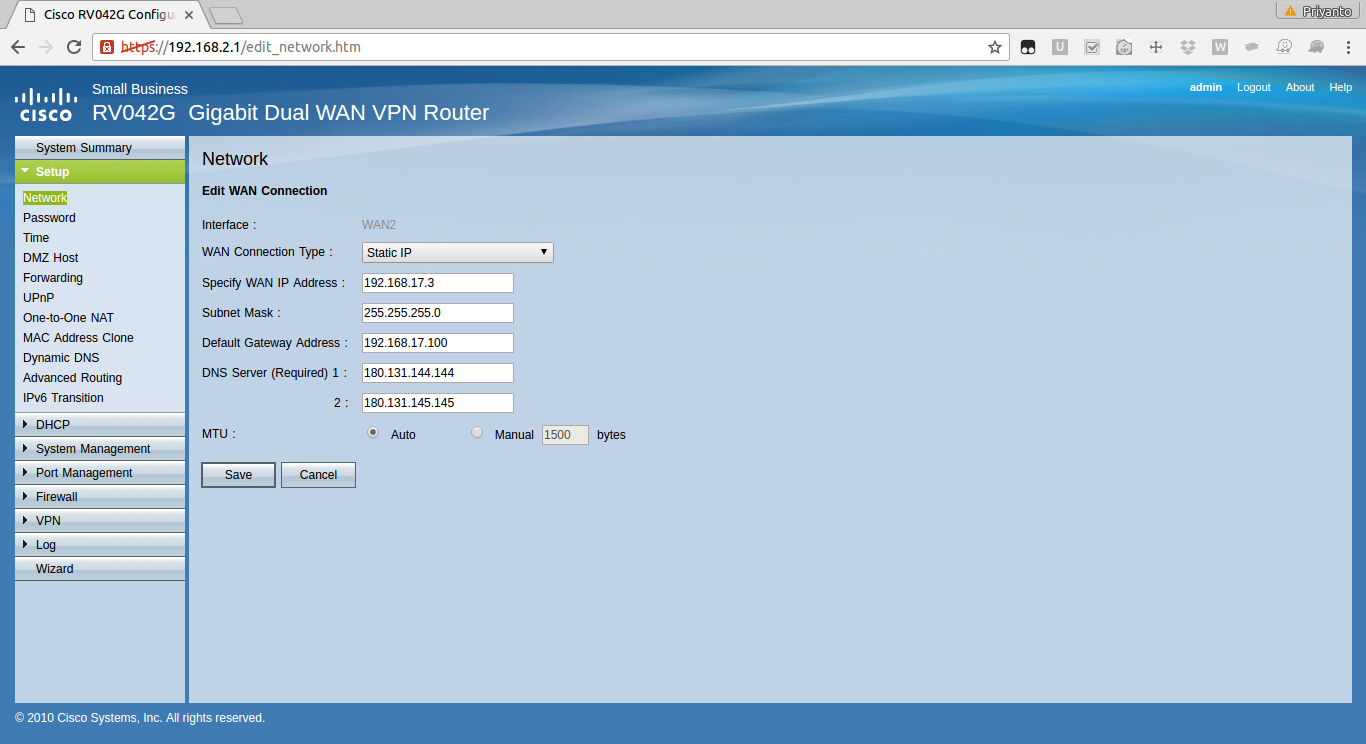
\includegraphics[width=1\textwidth]{./resources/konfig-cisco}
  \caption{Konfigurasi Cisco di WAN2}
  \label{fig:konfig-cisco}
\end{figure}

Agar \textit{client} di jaringan 17.0 dapat mengakses SISMIOP, maka diperlukan \textit{port forwarding} agar aplikasi SISMIOP dapat melakukan sambungan ke sistem basis data Oracle 11g. Konfigurasi \textit{port forwarding} untuk kasus ini adalah seperti pada gambar \ref{fig:port-forward-cisco} :

\begin{figure}[H]
  \centering
  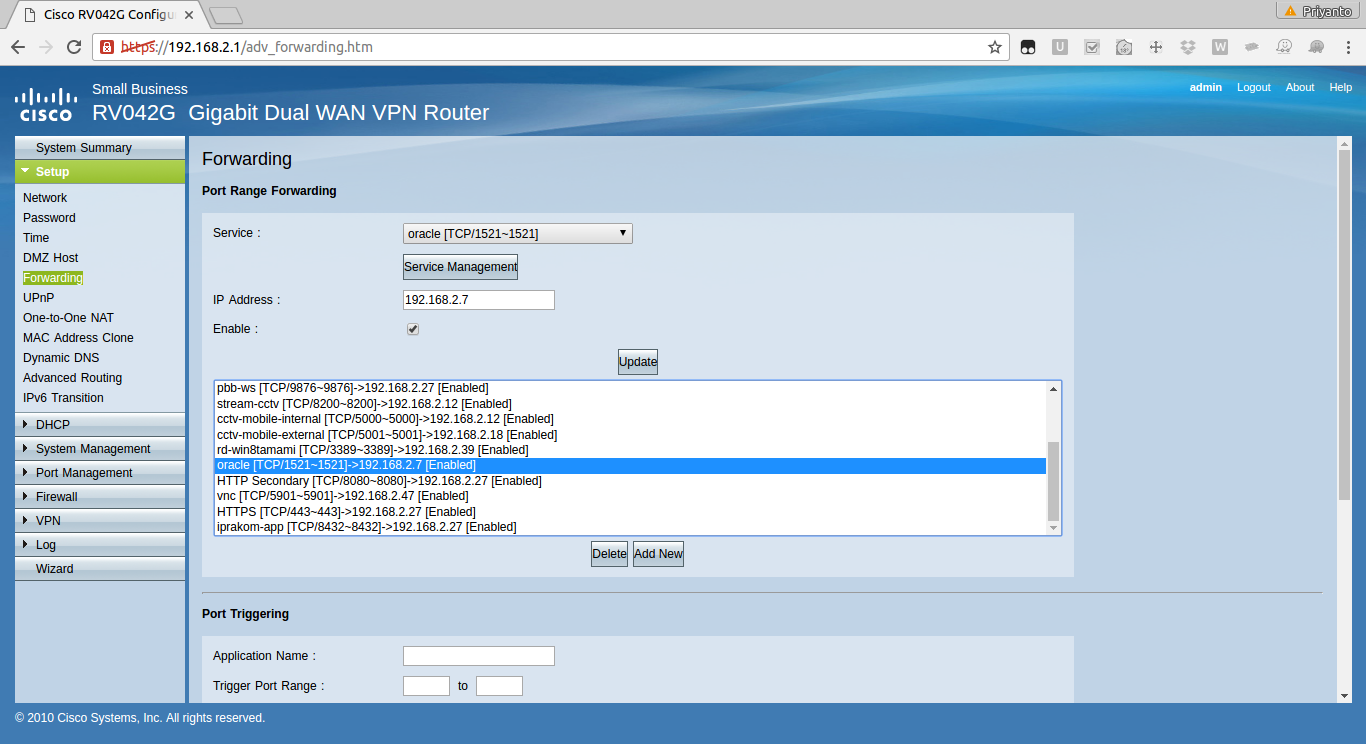
\includegraphics[width=1\textwidth]{./resources/port-forward-cisco}
  \caption{Konfigurasi Cisco Untuk \textit{Port Forwarding}}
  \label{fig:port-forward-cisco}
\end{figure}

\end{document}